
\section{Allgemein}
	\subsection{Schaltelemente bei zeitabhängigen Vorgängen}
	   		\begin{tabular}{p{1.5cm} p{4.3cm} |p{1.5cm} p{4.3cm}| p{1.5cm} p{4.3cm}}
	   	   		\multicolumn{2}{l}{\textbf{Ohmscher Widerstand R}}
	   	   			& \multicolumn{2}{l}{\textbf{Kapazitität C}}
	   	   			& \multicolumn{2}{l}{\textbf{Induktivität L}} \\
	   	   		\multicolumn{2}{l}{$u$ und $i$ können sprunghaft ändern}
	   	   			& \multicolumn{2}{l}{$\mathbf{u}$ \textbf{kann nicht sprunghaft ändern}}
	   	   			& \multicolumn{2}{l}{$\mathbf{i}$ \textbf{kann nicht sprunghaft ändern}} \\
	   	   	
	   	   		\multirow{2}{1.5cm}{
	   				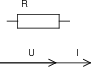
\includegraphics[width=1.5cm]{./bilder/zeigerdiag-r.png}}
	   				& $u(t) = R \cdot i(t)$ 
	   				& \multirow{2}{1.5cm}{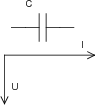
\includegraphics[width=1.5cm]{./bilder/zeigerdiag-c.png}}
	   				& $u(t) = \frac{1}{C} \int\limits_0^t i(\tau) d\tau + u(0)$
	   				& 
	   				\multirow{2}{1.5cm}{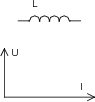
\includegraphics[width=1.5cm]{./bilder/zeigerdiag-l.png}}
	   				&$u(t) = L \frac{di(t)}{dt}$\\
	   				
	   				&$i(t) = \frac{u(t)}{R}$
	   				& & $i(t) = C \frac{d u(t)}{dt}$
	   				& & $i(t) = \frac{1}{L} \int\limits_0^t u(\tau) d\tau + i(0)$\\
	   				
	   				& $\underline{Z}_R = R$
	   				& & $\underline{Z}_C = \frac{1}{j \omega C} = - \frac{j}{\omega C}$
	   				& & $\underline{Z_L} = j \omega L$\\
	   	   	\end{tabular}
	   	
	   		\subsection{Vorgehen bei Schaltvorgängen}
	   		\fbox{$u(t) =U_E + (U_A - U_E) e^{\frac{-t}{\tau}} \qquad i(t) =I_E + (I_A - I_E) e^{\frac{-t}{\tau}} \qquad
	   		\tau = C R = \frac{L}{R}
	   		\qquad \underbrace{X_A}_{Anfang} = \lim\limits_{t
	   		 \rightarrow 0^+} x(t) \qquad \underbrace{X_E}_{Ende} =
	   		 \lim\limits_{t \rightarrow \infty} x(t)$} $\qquad$\\
	   		 \textbf{Beachte:} Spannung an $C$ und Strom an $L$ können nicht sprunghaft ändern. \\
	   		 Zur Bestimmung von R alle Quellen ausschalten und Belastung von Speicherelement her betrachten 
		 
		 
	\subsection{Vektor -/ Kreuzprodukt, Rechte-Hand-Regel}
	$\vec{c} = \vec{a} \times \vec{b}$: \qquad $\vec{c} \Leftrightarrow$ Daumen;
	$\vec{a} \Leftrightarrow$ Zeigefinger; $\vec{b} \Leftrightarrow$ Mittelfinger
	 
	\subsection{Matrixinversion einer 2x2-Matrix}
	$A^{-1} = \begin{bmatrix}
				a & b \\
				c & d \\
			\end{bmatrix}^{-1} = \frac{1}{\det(A)}
			\begin{bmatrix}
				d & -b \\
				-c & a \\
			\end{bmatrix} = \frac{1}{ad-bc}
						\begin{bmatrix}
							d & -b \\
							-c & a \\
						\end{bmatrix}$

	 \subsection{Partialbruchzerlegung\formelbuch{15}}
		Falls möglich, erst Polynomdivision.
		\[f(x)=\frac{x^2+20x+149}{x^3+4x^2-11x-30} \Rightarrow \; \begin{array}{l}\text{Nenner faktorisieren mit}\\
		\text{Hornerschema\formelbuch{914}, Binom, etc.}\end{array} \Rightarrow x^{3}+4x^{2}-11x-30=(x+2)(x^{2}+2x-15)=(8x+2)(x+5)(x-3)\]
		Ansatz:
		\[f(x)=\frac{x^2+20x+149}{x^3+4x^2-11x-30}=\frac{A}{x-3} + \frac{B}{x+2} + \frac{C}{x+5}=
		\frac{A(x+2)(x+5)+B(x-3)(x+5)+C(x-3)(x+2)}{(x-3)(x+2)(x+5)}\]
		Gleichungssystem aufstellen mit beliebigen $x_i$-Werten (am Besten Polstellen oder 0,1,-1 wählen):
		\[\begin{array}{l}x_1=3:\;-9+60+149=A\cdot5\cdot8\;\;\;\Rightarrow A=5\\
		x_2=-2:\;-4-40+149=B(-5)\cdot3\; \Rightarrow B=-7\\
		x_3=-5:\;-25-100+149=C(-8)(-3) \Rightarrow C=1 \end{array} \Rightarrow f(x)=\frac{5}{x-3}+\frac{7}{x+2}+\frac{1}{x+5}\]
		weitere Ansätze für andere Typen von Termen:
		\[f(x)=\frac{5x^2-37x+54}{x^3-6x^2+9x}=\frac{A}{x}+\frac{B_1}{x-3}+\frac{B_2}{(x-3)^2}=\frac{A(x-3)^2+B_1x(x-3)+B_2x}{x(x-3)^2}\]
		\[f(x)=\frac{1,5x}{x^3-6x^2+12x-8}=\frac{A_1}{x-2}+\frac{A_2}{(x-2)^2}+\frac{A_3}{(x-2)^3}=\frac{A_1(x-2)^2+A_2(x-2)+A_3}{(x-2)^3}\]
		\[f(x)=\frac{x^2-1}{x^3+2x^2-2x-12}=\frac{A}{x-2}+\frac{Bx+C}{x^2+4x+6}=\frac{A(x^2+4x+6)+(Bx+C)(x-2)}{(x-2)(x^2+4x+6)}\]
	\subsection {Komplexe Trigonometrie}
\begin{tabular}{lllllll}
$\sin{\underline{\alpha}} = \frac{e^{j\underline{\alpha}} - e^{-j\underline{\alpha}}}{2j}$ &

$\cos{\underline{\alpha}} = \frac{e^{j\underline{\alpha}} + e^{-j\underline{\alpha}}}{2}$ &

$\tan{\alpha} = \frac{\sin \alpha}{\cos \alpha}$ & 

$ \qquad \qquad $ &

$\sinh{\underline{\alpha}} = \frac{e^{\underline{\alpha}} - e^{-\underline{\alpha}}}{2} $ &

$\cosh{\underline{\alpha}} = \frac{e^{\underline{\alpha}} + e^{-\underline{\alpha}}}{2} $ &

		$\tanh(jb)=j \tan(b)$ 
\end{tabular}
							
	 